%!TEX root = booklet.tex

\section{Conference Venue: Beurs van Berlage}

When you enter from the street \emph{(Damrak 243)} and walk straight on, you will be in the \emph{Beursfoyer} \textbf{(0.3)}. To your right is the \emph{Grote Zaal} \textbf{(0.2)} ("zaal" stands for hall in Dutch; "kamer" stands for room). There, all breakfast, coffee breaks, lunches, afternoon demo/poster sessions as well as the PODS Reception on Sunday evening will be held. Also, all sponsor stands are located in the Grote Zaal. To your left are the \emph{Graanbeurszaal} \textbf{(0.5)} and the \emph{Effectenbeurszaal} \textbf{(0.4)}. Both are large halls, of which the latter will be used for all plenary sessions. Upstairs are the other, smaller, halls and rooms: \emph{Administratiezaal} \textbf{(1.1)}, \emph{Mendes da Costa kamer} \textbf{(1.2)}, \emph{Verwey kamer} \textbf{(1.4)}, \emph{Berlage zaal} \textbf{(1.9)}, \emph{Ontvangkamer} \textbf{(1.10)}, \emph{Veilingzaal} \textbf{(1.20)}.

%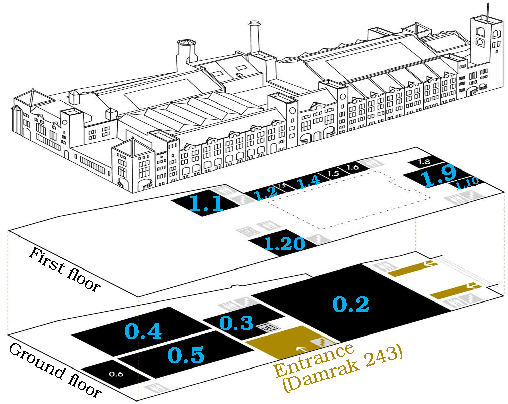
\includegraphics[width=\textwidth]{images/BvB-plan-3D-85mm-x-68mm.pdf}%
 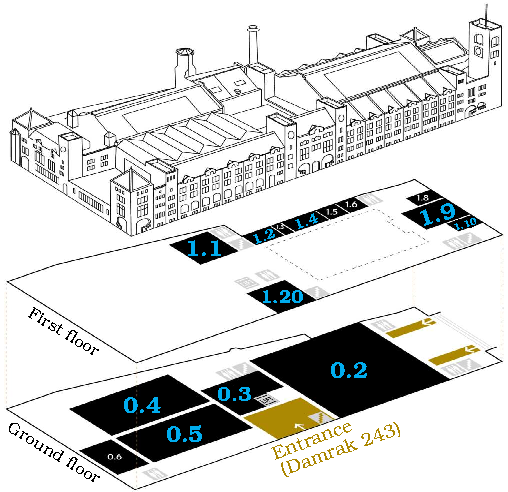
\includegraphics[width=\textwidth]{images/BvB-plan-3D-85mm-x-83mm.pdf}%

%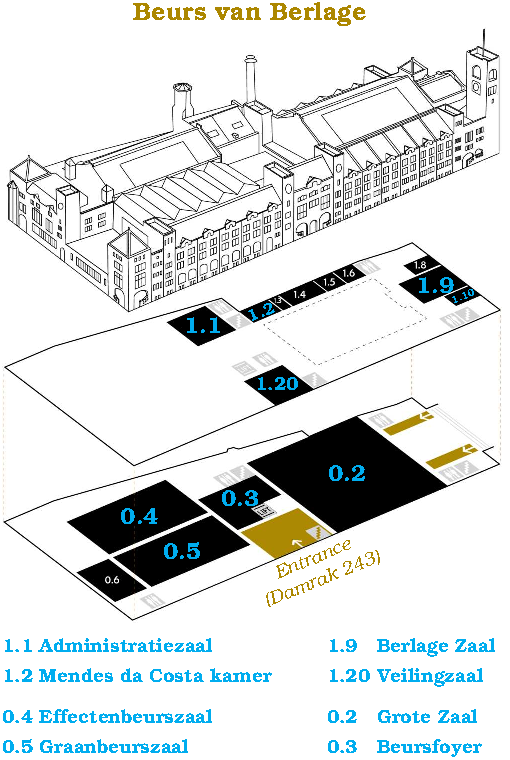
\includegraphics[width=\textwidth]{images/BvB-plan-3D-85mm-x-128mm.pdf}%

%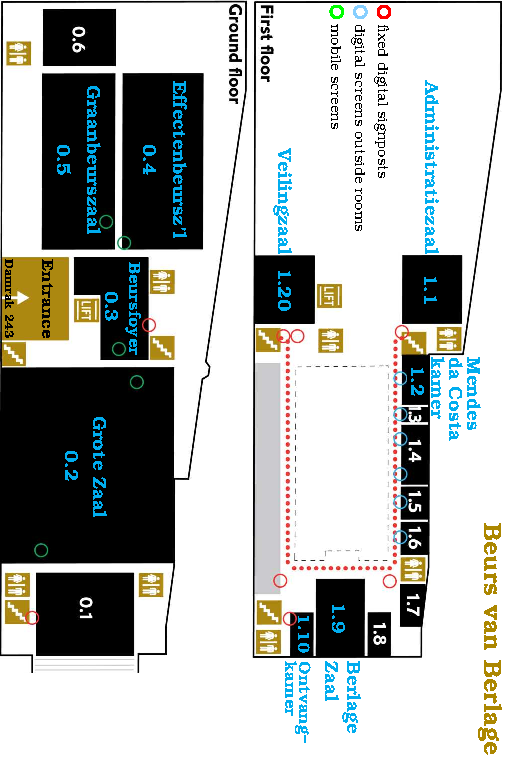
\includegraphics[width=\textwidth]{images/BvB-plan-2D-85mm-x-128mm-left.pdf}%

~
\vfill
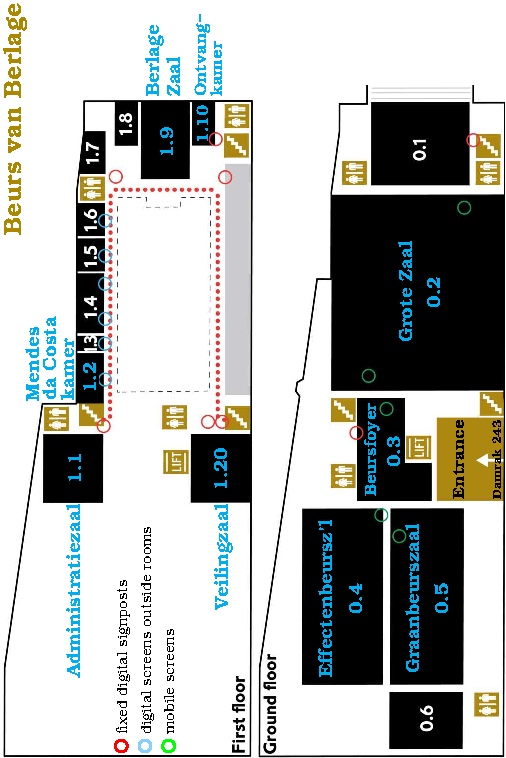
\includegraphics[width=.95\textwidth]{images/BvB-plan-2D-85mm-x-128mm-right.pdf}%

